% This is text associated with the open textbook "Open Electromagnetics"
% See immediately below for author, date
% This work is licensed under the Creative Commons Attribution-ShareAlike 4.0 International License. (CC BY-SA 4.0) 
% To view a copy of the license, visit http://creativecommons.org/licenses/by-sa/4.0/

%ORB TITLE Introduction to Transmission Lines
%ORB AUTHOR 0        # S.W. Ellingson, Virginia Tech (ellingson@vt.edu)
%ORB DATE 20180802   # yyyymmdd
%ORB ABSTRACT What we mean by "transmission line", role of wavelength, TEM vs. higher-order propagation modes

\label{m00028_Introduction_to_Transmission_Lines} % <-- Must match name of this file and module directory name.  Don't mess with this!

%ORB HIGHLIGHT
\begin{mdframed}[backgroundcolor=yellow!20,nobreak=true] 
A transmission line 
\index{transmission line!definition}
is a structure intended to transport electromagnetic signals or power.
\end{mdframed}
%
A rudimentary transmission line is simply a pair of wires with one wire serving as a datum (i.e., a reference; e.g., ``ground'') and the other wire bearing an electrical potential that is defined relative to that datum. 
Transmission lines having random geometry, such as the test leads shown in Figure~\ref{m0028_fPoorTL}, are useful only at very low frequencies and when loss, reactance, and immunity to electromagnetic interference (EMI) 
\index{electromagnetic interference (EMI)}
are not a concern.
%
\begin{figure}[b!]
\begin{center}
\pdftooltip{{  % note double braces
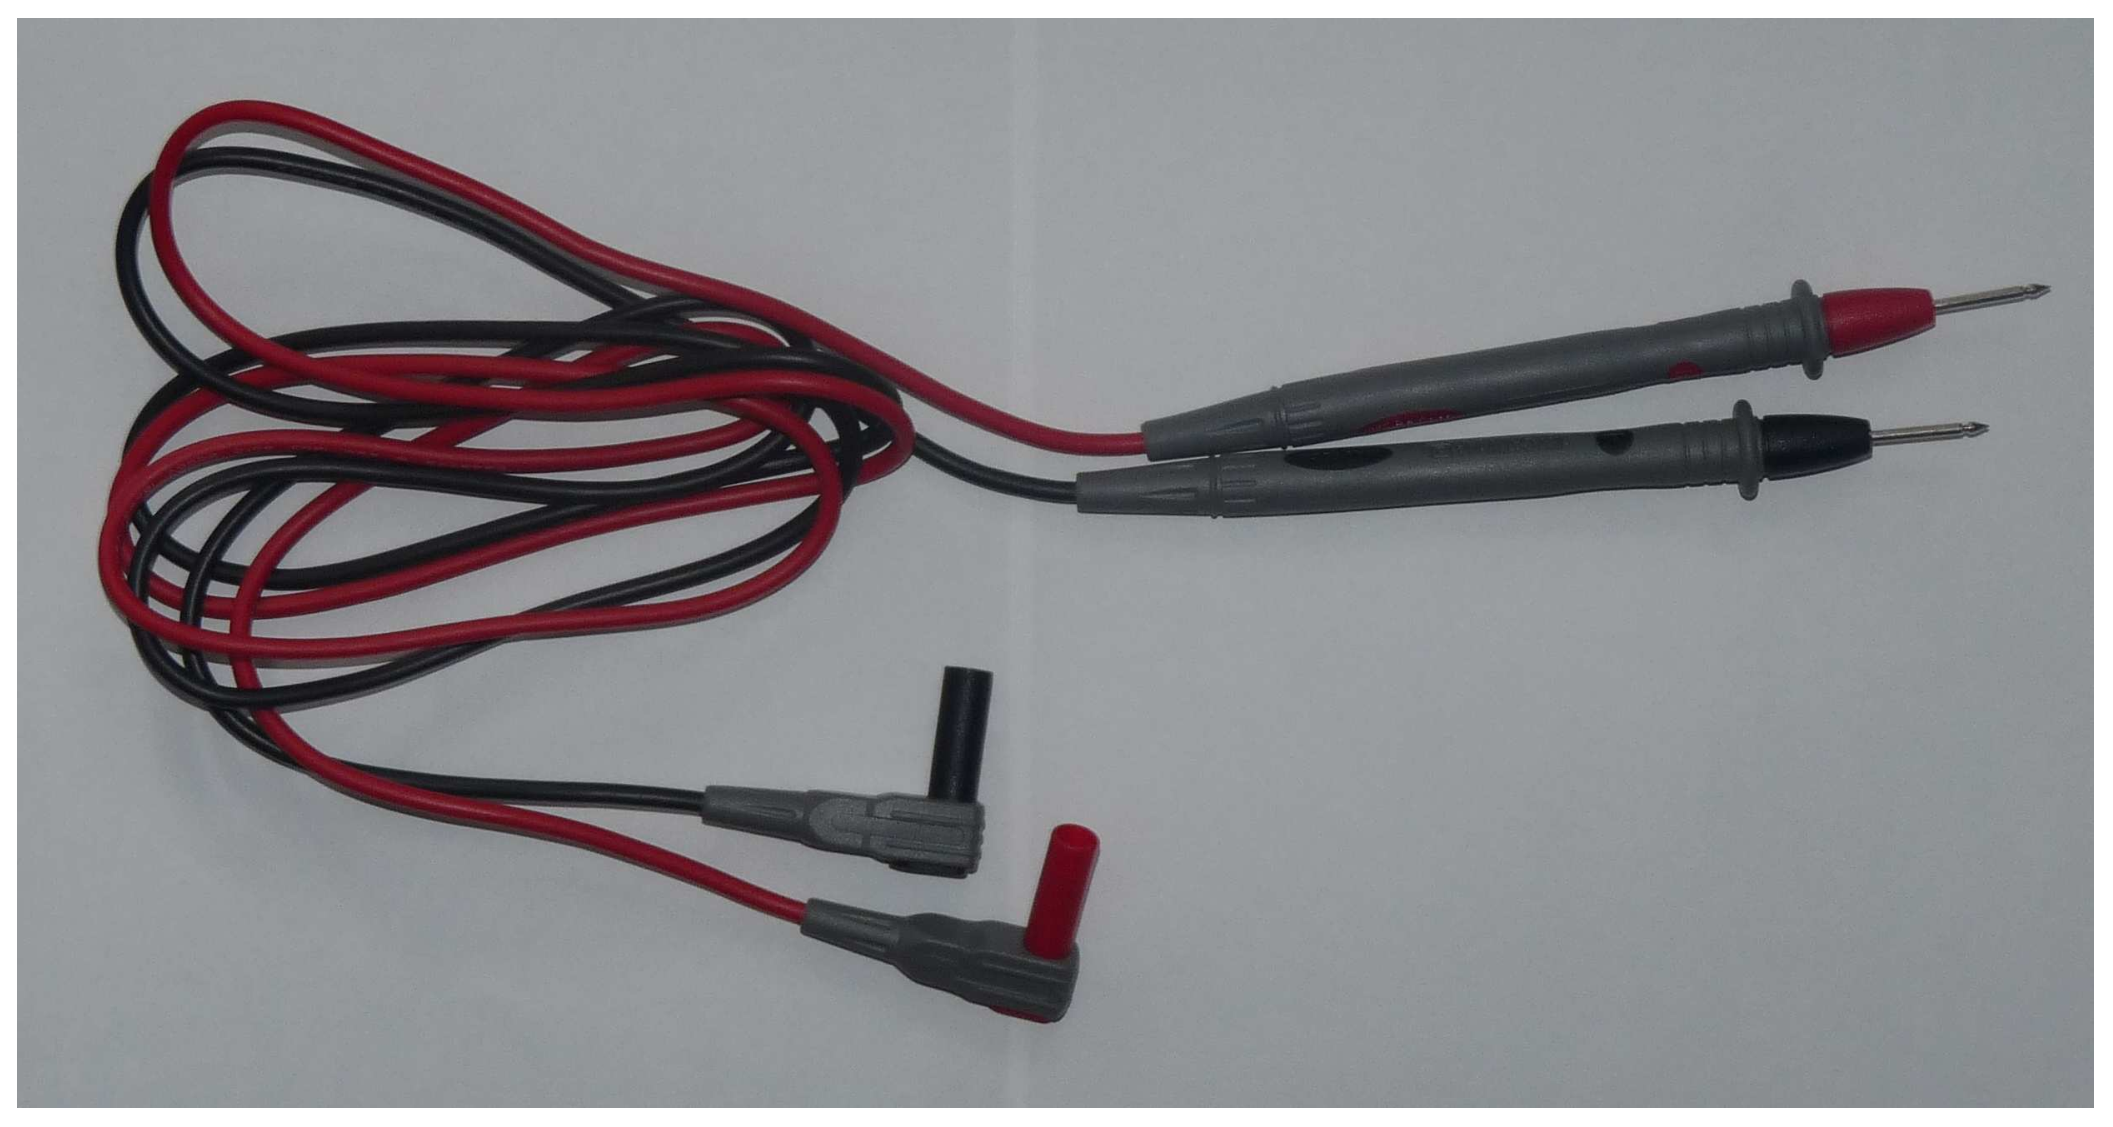
\includegraphics[width=\columnwidth]{modules/m0028_fMastech_test_leads.eps}
}}{Image of a set of electrical test leads. Each lead is comprised of a connector that fits the voltmeter and a tubular section with a pointed metal tip. The connector and metal probe tip are connected by wire. One lead is red and one is black.}
\end{center} 
%\vspace{2in}
% https://en.wikipedia.org/wiki/File:Mastech_test_leads.JPG
\centerline{\scriptsize 
by~\hyperref[m0028_fPoorTL_Credit]{Dmitry~G}
% public domain
}
\caption{
\label{m0028_fPoorTL}
These leads used to connect test equipment to circuits in a laboratory are a very rudimentary form of transmission line, suitable only for very low frequencies.
}
\end{figure}

However, many circuits and systems operate at frequencies where the length or cross-sectional dimensions of the transmission line may be a significant fraction of a wavelength. In this case, the transmission line is no longer ``transparent'' to the circuits at either end.
Furthermore, loss, reactance, and EMI \emph{are} significant problems in many applications.
These concerns motivate the use of particular types of transmission lines, and make it necessary to understand how to properly connect the transmission line to the rest of the system.

In electromagnetics, the term ``transmission line'' refers to a structure which is intended to support a \emph{guided wave}.
\index{waves!guided}
A guided wave is an electromagnetic wave that is contained within or bound to the line, and which does not radiate away from the line.  
This condition is normally met if the length and cross-sectional dimensions of the transmission line are small relative to a wavelength -- say $\lambda/100$ (i.e., 1\% of the wavelength). 
For example, two randomly-arranged wires might serve well enough to carry a signal at $f=10$~MHz over a length $l=3$~cm, since $l$ is only 0.1\% of the wavelength $\lambda=c/f=30$~m.  
However, if $l$ is increased to $3$~m, \emph{or} if $f$ is increased to 1~GHz, then $l$ is now 10\% of the wavelength.
In this case, one should consider using a transmission line that forms a proper guided wave. % that is not prone to unintended radiation. 

Preventing unintended radiation is not the only concern.
Once we have established a guided wave on a transmission line, it is important that power applied to the transmission line be delivered to the circuit or device at the other end and not reflected back into the source.
For the random wire $f=10$~MHz, $l=3$~cm example above, there is little need for concern, since we expect a phase shift of roughly $0.001\cdot 360^{\circ} = 0.36^{\circ}$ over the length of the transmission line, which is about $0.72^{\circ}$ for a round trip.  So, to a good approximation, the entire transmission line is at the same electrical potential and thus transparent to the source and destination.
However, if $l$ is increased to $3$~m, \emph{or} if $f$ is increased to 1~GHz, then the associated round-trip phase shift becomes $72^{\circ}$.  In this case, a reflected signal traveling in the opposite direction will add to create a total electrical potential, which varies in both magnitude and phase with position along the line. 
Thus, the impedance looking toward the destination via the transmission line will be different than the impedance looking toward the destination directly.
(Section~\ref{m0087_Input_Impedance_of_a_Terminated_Lossless_Transmission_Line} gives the details.)
The modified impedance will depend on the cross-sectional geometry, materials, and length of the line.  
     
Cross-sectional geometry and materials also determine the loss and EMI immunity of the transmission line.  

Summarizing:
%
%ORB HIGHLIGHT
\begin{mdframed}[backgroundcolor=yellow!20,nobreak=true] 
Transmission lines are designed to support guided waves with controlled impedance, low loss, and a degree of immunity from EMI. 
\end{mdframed}



